\documentclass[11pt]{article}

\usepackage[T1]{fontenc}
\usepackage{geometry}
\usepackage{microtype}

\usepackage{newtxmath}
\usepackage{newtxtext}
\usepackage{graphicx}

\usepackage{xcolor}
\definecolor{cobalt}{rgb}{0.0, 0.28, 0.67}

\newenvironment{resp}{\begin{quote}\color{cobalt}}{\end{quote}}
\newcommand{\sresp}[1]{\textcolor{cobalt}{#1}}

\setlength{\parindent}{0in}
\setlength{\parskip}{11pt}

\title{Response to peer reviews}
\author{}
\date{\today}

\begin{document}
\maketitle


\section*{Editor}


  Reviews are generally supportive, but bring up several issues that need to be
  addressed. Once addressed, please submit the revised manuscript with an
  item-by-item reply/rebuttal.  


\begin{resp}
  We thank the editor and reviewers for their comments and the opportunity to make
  revisions. We have made a number of revisions, described in detail below.
  We believe these changes have strengthened the manuscript, and describe them in
  more detail below.
  We quote below the Reviewer comment and provide our response in this color.
\end{resp}


\section*{Reviewer 1}



  1. In their presentation of of evaluation metrics they do not discuss
  stability. For instance in [7] does the choice of the weights, using $\tau$ for
  $x\geq 0$ rather than some monotone function say some power $\tau^\alpha$ make a
  difference? Since as they indicate the measure is used for fitting as well as
  ascertainment, some stability investigation seems appropriate. I suspect here
  is no great effect but...


\begin{resp}
  The reviewer is correct: the choice of $\tau$ rather than a monotone function of
  $\tau$ will make a difference. But it seems that we should have been more clear
  in our description of WIS. The weights used here are those used to evaluate
  forecasts submitted to the COVID-19 Forecast Hub and the CDC. More broadly,
  this is a standard metric in the forecasting community (just as Mean Squared
  Forecast Error is standard), rather than an ``author decision''.  With the
  weights as used, it is equivalent to quantile loss and therefore is a discrete
  version of CRPS (see [7]).

  In principle,
  we would expect that different weights may alter the conclusions, though
  likely not substantively. Applying a monotone function to $\tau$ only effectively
  changes the quantile of interest, resulting in a mismatch between the coverage you
  tried to get and the coverage WIS is evaluating. Applying the function to $\tau$
  and $(1-\tau)$ results in an asymmetry, penalizing forecasts that miss on one
  side more than on the other.

  $\bullet$ We have added a sentence in the Evaluation Metrics section emphasizing that
  this metric is standard.
\end{resp}


  2. They do not discuss the possible effects of vaccination rates and other
  factors, though this may be one of the areas of localization they propose to
  investigate.



\begin{resp}
  During the period discussed in the main paper, vaccinations had essentially no
  effect. On Dec 31 2000, when the main evaluation period ends,  according to
  CDC data, about 1\% of the population 
  had received 1 dose. That said, we should probably be more specific in the
  paragraph on lines 31-40: our goal is to use very simple models that do not
  account for extra information (vaccinations but also strains of the virus,
  ``super-spreader'' events, etc.).

  $\bullet$ We have added a sentence around lines 30--40 emphasizing the choice
  to ignore such factors.
\end{resp}


  3. This points to what is perhaps a more major issue. Can they identify in
  quantitative terms the consequences of the additional improvements in
  forecasting provided by these methods in terms of gains in resources available
  to deal with the epidemic? Unfortunately as they state, in the crucial periods
  of sharply rising cases, the additional benefit seems least.


\begin{resp}
  This is a good point, and we have made a few modifications described in more
  detail below (Reviewer 2, Point 3).
\end{resp}



  4. Despite the fact that a detailed description of terms in the text is
  impossible, it would I think be helpful to say if there is any significance to
  the names they associate with their first 2 and 4th indicators.


\begin{resp}
  It seems that the Reviewer is referring to CHNG-CLI, CHNG-COVID and DV-CLI. These are
  described in the Methods Section, Signals and Locations Subsection. To be more
  specific, Change 
  Healthcare is a large healthcare insurance claims processor. The difference
  between ``-CLI'' and ``-COVID'' is that the first measures insurance
  claims involving symptoms
  associated with COVID-like-illness  while the second requires a medical
  diagnosis (through 
  testing or presumed positive by the medical provider). The ``DV'' modifier
  corresponds to different claims processors (not Change Healthcare) who wish to
  remain anonymous.

\end{resp}



  5. What are Change Healthcare claims..as opposed to others?


\begin{resp}
  Hopefully the discussion to point 4 above has cleared up any confusion.
\end{resp}


\section*{Reviewer 2}
\begin{quote}
  \emph{(items numbered by the editor for convenience of reference)}
\end{quote}

\subsection*{Statistical or Methodological Comments:}
  
1. Is this really a stationary phenomenon? Over the timerange extending from
pre-lockdown to today, it certainly isn't. The method in this paper of
presenting model prediction errors makes it impossible to see this. People in
econometrics look at cumsums of normalized prediction errors. You can see change
points and trends very easily.

\begin{resp}
  There is little reason to believe that this data is stationary. The models
  however are trained and evaluated over reasonably short periods (2-3 months),
  over which time the behavior may well be stationary. We have added a section
  to the appendix that uses the cumulative sum normalized by baseline as
  suggested. With some exceptions at the beginning of 
  the evaluation period, the relative ordering remains fairly consistent. The AR
  model is easily the worst.

\end{resp}

2. Are the results in this paper statistically significant? I see no discussion
of this question, which seems unbelievable for me to be saying, given the
authorship. And yet here I am.

\begin{resp}
  As noted in the introduction, there are no options available for fully 
  rigorous and nonparametric (model-free) statistical significance testing,
  giving the intricate spatiotemporal dependence in our forecasting problem.  

  We also have strong reasons for not using model-based approaches (in part due
  to nonstationarity, but also due to the belief that these models are not
  applicable here). We felt that our extensive predictive comparisons in the
  methods section and supplement were more appropriate. 

  That said, to address this more directly we have made a number of additions: 

  $\bullet$ We have added a section to the Supplement (and point
  to it around 
  line 458 in the main text), that performs a Sign Test for differences in
  accuracy. P-values there tend to cluster near zero and one suggesting some
  periods have significantly improved accuracy for the indicator-assisted models
  while in others, the reverse is true.

  $\bullet$ We also use a Diebold-Mariano test
  for comparing forecast accuracy. The results for this test are mixed, as would
  be expected given the sign test and
  the nonstationarity the Reviewer mentions above. The indicators are
  more helpful in some periods than others, see also the upswing/downswing
  discussion in Section 2C. 
\end{resp}

3. Are the results in this paper practically significant? I see no discussion of
this question, which seems unbelievable for me to be saying, given that the
authors refuse to consider statistical significance. And yet here I am.

\begin{resp}
  See also Reviewer 1 point 3. And the general comment below (Point 8) where we
  outline some specific changes we have made that bare on this point.
  
  Practically, on average, if our goal is to predict 11 days ahead, when the AR
  model is at its best, CHNG-CLI
  doesn’t help (at least with these simple models). However, CHNG-COVID,
  DV-CLI, and Google-AA ``buy'' 4 extra days for the 
  same accuracy. CTIS-CLIIC ``buys'' about 5 extra days. What we mean here is
  that if we have a certain tolerance for inaccuracy, adding these signals increases the
  horizon at which we can predict within our tolerance. As for the
  practical significance of 4-5 extra days, this would of course depend on the use case.  However, cases grow
  exponentially, so making public policy changes 15 or 16 days ahead rather than
  11 can mean real gains. There also seems to be a fairly constant mapping
  between cases and future hospitalizations. Giving
  hospitals a few extra days to accumulate supplies and find personnel is
  meaningful. For predicting hotspots, we see similar results (gains of a few
  days) though with different indicators. 
\end{resp}

4. For the cumsum plots I mentioned above, and other related techniques, we can
plot all the model prediction error cumsum curves versus time and thereby
compare different models for size, nonstationarity and significance of
prediction improvement. The plots that have been presented in Figure 4 say do
none of those tasks.

\begin{resp}
  We added the cumulative-sum plot as described above. Additionally, the
  Reviewer's point aligns with much of  our motivation for Fig 4. If we were
  predicting a single location's 
  time series, then the cum-sum plot would provide all the information.
  However, we have a separate time series prediction problem for each HRR, and
  the upswings/downswings occur at different dates in different HRRs, so
  conditioning on forecast date for the comparison (as is done in a
  cumulative-sum plot) ends up adding together errors from different phases
  of the pandemic. In Figure 4, we instead condition on phase of the pandemic,
  which we think is more meaningful than calendar date. 
\end{resp}

5. The idea of using Asof data is of course important but I have known about it
for twenty years and practiced it routinely; it has apparently been in routine
use in econometrics for 40 years.

\begin{resp}
  We appreciate the Reviewer's perspective on the ubiquity of Asof data in
  econometrics. But the epidemic modelling community is less aware. And it
  has a real and meaningful importance for model selection going forward. We
  hope that this paper will lead to greater appreciation of this issue in this
  community. 
\end{resp}

\subsection*{Comments on Significance Statement:}

6. I don't know what ``all provide a nontrivial boost in accuracy'', really
means. I guess that the general audience won't either.

\begin{resp}
  We have changed the clause to ``all provide a nontrivial improvement in
  forecast accuracy''
\end{resp}

7. The sentence following is missing a word: depends ***on*** the pandemic...

\begin{resp}
  Fixed. Thank you for catching this.
\end{resp}

\subsection*{General Comments: }

8. In my understanding there are some standard models which have been relied
upon I guess millions of times during the pandemic. For example IHME's model.
The authors say a sentence or so about their choice of baseline, saying what
seems to me quite vague about the relation between their baseline and the
heavily used existing models. Wouldn't it be better to identify a specific
widely-used model explicitly as a baseline and then develop measures of
improvement over that specific widely used model? Also, might the authors
explain how the improvements observed by the authors stack up in terms of
concrete differences over the widely used models that people have been using.
Are there major misses that have taken place and could have been avoided?  


\begin{resp}
  We have tried to focus mainly on simple time series models in this paper
  rather than comparing to other more elaborate models. A careful
  (out-of-sample) comparison of forecasting performance for state-of-the-art
  models can be found in reference 6 (Cramer et al.). That paper focuses on
  forecasting deaths rather than cases and at the state-level rather than
  disaggregated HRRs. However, their ranking (Figure 2 of Cramer et al.) puts the
  ``COVIDhub-Baseline'' about 10th out of 27 models. As we discuss in the
  manuscript, that baseline is  
  the
  same as the baseline we use for forecasting in this paper: it propagates today
  forward and resamples the residuals to create quantiles (we have expanded the
  description on page 6 to be more explicit). All our ``simplistic'' models beat
  this baseline (the AR(3) does as well). For comparison, IHME (along with 17 other
  ``state-of-the-art'' models) does not. We would argue that using any of the
  models in this paper would be preferable to relying on many of the
  ``widely-used'' models if the goal is forecast accuracy.

  $\bullet$ We have added a sentence to the introduction (around line 40) that
  describes the performance of simple models relative to widely-used models as
  shown in Cramer et al.

  $\bullet$ We have expanded our description of our baseline model (around line
  457). In particular, we emphasize that it is the same as that used by the
  COVID-19 Forecast Hub.

  $\bullet$ To directly address the Reviewer's point about IHME, we include two
  figures here
  that compare our forecasts with state-of-the-art forecasts
  submitted to the COVID-19 Forecast Hub. The first overlays the
  scores from the submissions on top of Figure 3 from the manuscript. We should
  note that the submitted forecasts are at the state level, while ours are at
  the HRR level, but once scaled by the baseline, should be roughly comparable.
  Only those forecasters that submitted at least 300 forecasts (roughly 50
  states over 6 weeks during the 6 months examined) are shown. From this Figure
  it is clear that all of the forecasters considered in this paper beat most
  submissions. In the second figure, we use the Geometric Mean scaled by the
  baseline as shown in Figure S6 in the Supplement. By this metric, the methods employed in this
  paper would rank in the top 2 of all submitted forecasts, beating the
  COVIDhub-ensemble at all forecast 
  horizons. The improvement of the best indicator assisted model over the AR model
  is roughly the same as the improvement of the AR model over the
  COVIDhub-ensemble.

  \begin{figure}[tb]
    \centering
    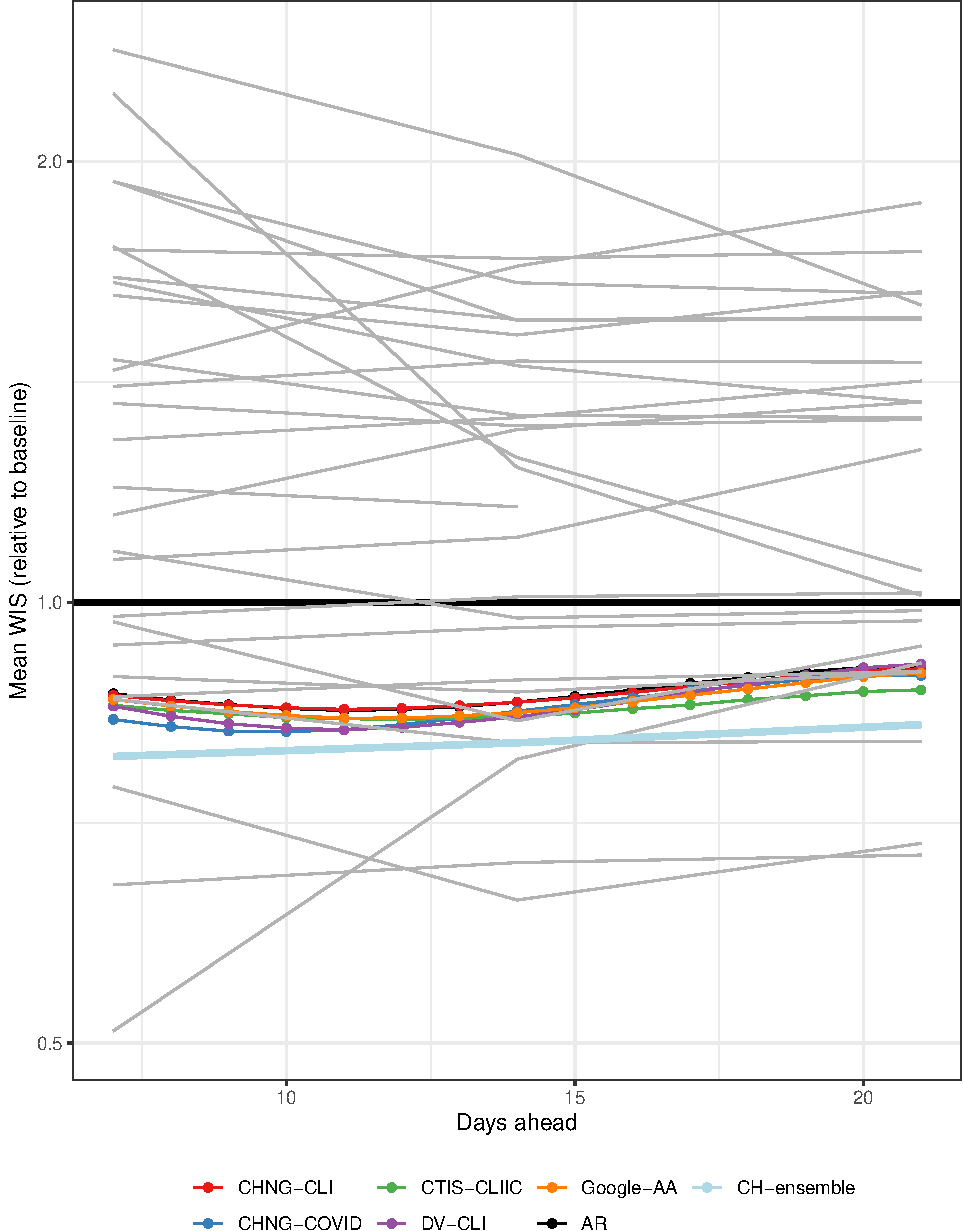
\includegraphics[width=.9\textwidth]{fig/compare-to-hub-mean-1.pdf}
    \caption{This figure reproduces Figure 3 in the main paper but overlays
      scores for the forecasts submitted to the COVID-19 Forecast Hub. Grey
      lines correspond to the various teams that submitted during period our
      evaluation period. We have highlighted the COVIDhub-ensemble, which is the
      official forecast of the CDC.}
    \label{fig:compare-to-hub-mean}
  \end{figure}

  \begin{figure}[tb]
    \centering
    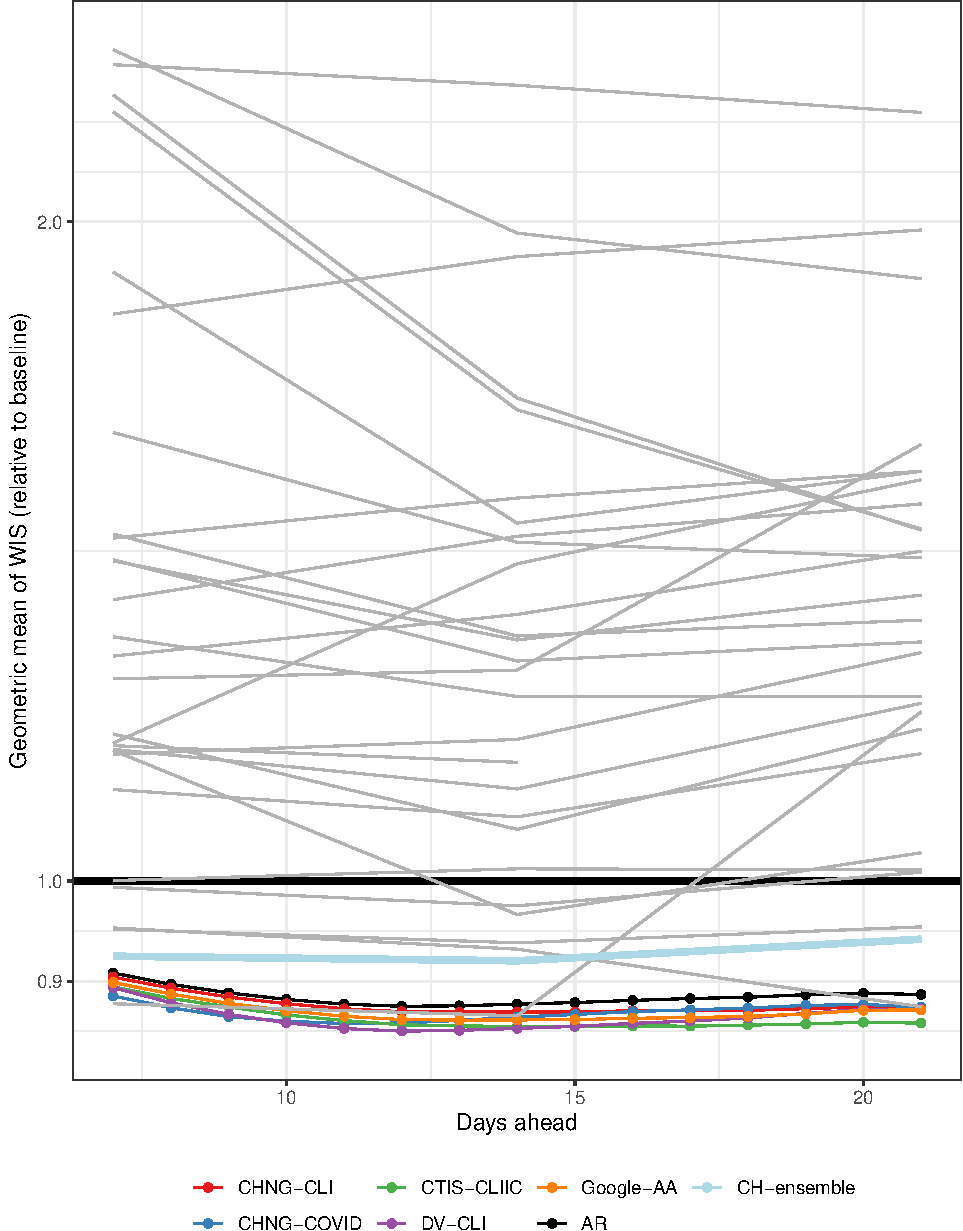
\includegraphics[width=.9\textwidth]{fig/compare-to-hub-geomean-1.pdf}
    \caption{This figure is more like Figure S6 in the Supplement. In this case,
      we add 1 to both the forecaster WIS and the baseline WIS before scaling
      (to allow forecasters that achieve 0 error to appear), and we overlay
      scores for the forecasts submitted to the COVID-19 Forecast Hub. Grey
      lines correspond to the various teams that submitted during period our
      evaluation period. We have highlighted the COVIDhub-ensemble, which is the
      official forecast of the CDC.}
    \label{fig:compare-to-hub-geomean}
  \end{figure}
\end{resp}


\end{document}